\documentclass[border=5mm]{standalone}
\usepackage{tikz}
\begin{document}
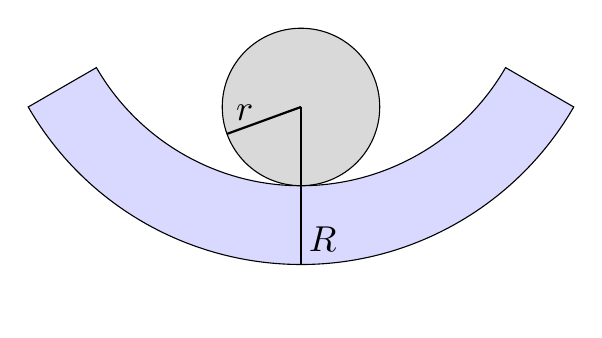
\begin{tikzpicture}[
  every node/.style={scale=1.3}
]
% inner/outer circle:
% sadly the length of the outer circle is only roughly approximate
\filldraw [fill=gray!30, draw=black] (0,0) circle[radius=1];
\filldraw[fill=blue!15, draw=black, shift={(0,2)}] (330:3) arc (330:210:3) -- (210:4) arc (210:330:4) -- cycle;
\draw [thick] (0,0) -- (-160:1cm) node[anchor=230] {$r$};
\draw [thick] (0,0) -- (-90:2cm) node[anchor=230] {$R$};
\end{tikzpicture}
\end{document}